% The original template for ICIP-2000 paper; to be used with:
%          spconf.sty  - ICASSP/ICIP LaTeX style file, and
%          IEEEbib.bst - IEEE bibliography style file.
% --------------------------------------------------------------------------
\documentclass{article}
\usepackage{spconf,amsmath,epsfig,url}
\usepackage{verbatim}
% Example definitions.
% --------------------
\def\x{{\mathbf x}}
\def\L{{\cal L}}

% Title.
% ------
\title{NLP Project}
%
% Single address.
% ---------------
\name{Student A,}
\address{Department of Computer Engineering\\ Chulalongkorn Univerisy\\ Bangkok, Thailand}

% For example:
% ------------
%\address{School\\
%		 Department\\
%		 Address}
%
% Two addresses (uncomment and modify for two-address case).
% ----------------------------------------------------------
%\twoauthors
%  {A. Author-one, B. Author-two\sthanks{Thanks to XYZ agency for funding.}}
%		 {School A-B\\
%		 Department A-B\\
%		 Address A-B}
%  {C. Author-three, D. Author-four\sthanks{The fourth author performed the work
%		 while at ...}}
%		 {School C-D\\
%		 Department C-D\\
%		 Address C-D}
%
\begin{document}
%\ninept
%
\maketitle
%
\begin{abstract}
Describe in concise words what you do, why you do it (not necessarily
in this order), and the main result.  The abstract has to be
self-contained and readable for a person in the general area. You
should write the abstract last.
\end{abstract}

\section{The report should include at least} \label{sec:we_must_do}
    \begin{itemize}
  \item  Information about the data and data statistics
  \item Information about the model and techniques used including model training time
  \item  Experiments done + Error analysis
  \item Lessons learned or insights gained
  \item  Information about the demo system (if any)
  \item Manual on how to use the code/model
\end{itemize}

\section{Introduction}\label{sec:intro}

Do not start the introduction with the abstract or a slightly modifed
version.

\subsection{Motivation}

Start with the general setup of your paper. Where does the problem you
address come from and what is the motivation. The motivation is very
important.
% ในการเขียนบทความต่างๆนั้น การเขียนสิ่งที่มีความหมายเดิมเรา
\subsection{Previous Work}

Describe related work relevant to this paper. Make clear what was
done and what was not done. \cite{ma2018query} \cite{sennrich2016edinburgh}
% paper ที่เกี่ยวกับ seqtoseq
\subsection{What I Am Going to Do}

Explain what you do, in a readable way, how you do it, and the main
results you obtained. For a real paper, you would also make very clear
here what is novel about your contribution. Also, you can reiterate
why your work is relevant.

\subsection{Organization of the Paper}

Give a one paragraph overview of the paper, like: In
Section~\ref{sec:background} we provide the background on the the
discrete Fourier transform and its most important fast algorithms
including their detailed cost analysis. In ...

\subsection{General Comments}

\begin{itemize}
\item You do not have to follow the exact subsection titles in this section
or the others. It is just to help you get started.  Alternatively, and
what I usually do to save space, is to use paragraph titles instead of
subsections, as in

{\bf Organization of the paper.} Blabla.

\item It is generally a good idea to break sections into smaller units for
readability and since it helps you to structure the story.

\item Also, the following section titles should be adapted to more precisely
reflect what you do.

\item It is helpful to start each of the following sections with a very
short summary of what the reader can expect in the section. Nothing
more awkward as when the story starts and one does not know what the
direction is or the goal.

\item Make sure you define each acronym you use, no matter how convinced you are
the reader knows it.

\item Always spell-check before you submit (to me in this case).

\item Be picky. When writing a paper you should always strive for very
high quality. Many people may read it and the quality makes a big difference.

\item Books helping you to write better: \cite{Higham:98} and \cite{Strunk:00}.

\item Conversion to pdf (latex users only): 

dvips ... -Ppdf -G0 ....
\end{itemize}


\section{Necessary Background}
\label{sec:background}

Here you should give a short, self-contained summary of necessary
background information. For example, assume you present about reinforcement learning. You could organize into reinforcement learning basics, the Bellman equation, and how to train a model.

\subsection{Seq2seq key-value attention}

\subsection{Seq2seq Bahdanau attention}

\subsection{Model training}

{\bf Note: You have to:}
\begin{itemize}
\item Seq2seq key-value attention				
\begin{itemize}
\item Encode
\begin{itemize}
\item Bidirectional LSTM
\end{itemize}
\end{itemize}
\begin{itemize}
\item Decoder
\begin{itemize}
\item Attention (Key-Value) Homework 8
\end{itemize}
\begin{itemize}
\item LSTM
\end{itemize}
\end{itemize}
\end{itemize}

\begin{itemize}
\item Seq2seq Bahdanau attention				
\begin{itemize}
\item Encode
\begin{itemize}
\item GRU
\end{itemize}
\end{itemize}
\begin{itemize}
\item Decoder
\begin{itemize}
\item Bahdanau Attention 
\begin{itemize}
\item(Bahdanau et.,al 2018v7)
\end{itemize}
\end{itemize}
\begin{itemize}
\item GRU
\end{itemize}
\end{itemize}
\end{itemize}



\section{Your Proposed Method}\label{sec:yourmethod}

Here you explain what you did, again first starting with a brief overview.
Structure it as suitable. 

{\bf Note: You have to:}
\begin{itemize}
\item Explain all steps you performed so that another person can re-produce your experiments as close as possible
\item This can be exactly like the paper you try to replicate. However, you should try to explain it it your own words. Most paper has space constraints and left out many details and hyperparameter choices. Describe what you use.
\end{itemize}



\section{Datasets} \label{sec:data}

\begin{itemize}
\item Opusparcus: Open Subtitles Paraphrase Corpus for Six Languages 
\item \url{https://korp.csc.fi/download/opusparcus/}
\end{itemize}
\begin{center}
 \begin{tabular}{||c c ||} 
 \hline
First Sentence & Second Sentence \\ [0.5ex] 
 \hline\hline
 You're not alone , Claire . & You are not alone , Claire . \\ 
 \hline
 Jumby now wants to be born . & Jumby want birth .  \\ [1ex] 
 \hline
\end{tabular}
\end{center}


\section{Experimental Results} \label{sec:exp}
\subsection{model}
USE 3 MODEL
\begin{itemize}
\item Seq2seq key-value attention
\item Seq2seq Bahdanau attention
\item Tranformer
\end{itemize}


\subsection{evaluation}
{\bf Evaluation: BLEU score}


\begin{itemize}
\item Seq2Seq KV-Attention
\begin{itemize}
\item BLEU AVG : 21.25
\item BLEU MAX : 28.66
\item BLEU MIN : 0.00
\end{itemize}
\end{itemize}

\begin{itemize}
\item Seq2Seq Bahdanau Attention
\begin{itemize}
\item BLEU AVG : 27.76
\item BLEU MAX : 75.98
\item BLEU MIN : 0.00
\end{itemize}
\end{itemize}

{\bf Didn’t work model : Transformer(Cont.)}


\begin{itemize}
\item Seq2Seq Transformer Encoder (Word Base)
\begin{itemize}
\item BLEU AVG : 19.31
\item BLEU MAX : 100.00
\item BLEU MIN : 0.00
\end{itemize}
\end{itemize}

\begin{itemize}
\item Seq2Seq Bahdanau Attention (Char Base)
\begin{itemize}
\item BLEU AVG : 17.05
\item BLEU MAX : 100.00
\item BLEU MIN : 0.00
\end{itemize}
\end{itemize}

\subsection{Error analysis}
% จากตัวของ dataset ที่เราได้มานั้น


\section{Conclusions} \label{sec:conclusion}

You can reference a paper by creating a key-value pair in conference.bib (at the bottom of the file, see example file). The format of the citation information follows bibtex format. Most journal websites or google scholar have a section where you can easily copy and paste the bibtex of the paper (see Figure \ref{fig:bibtex}). To cite, just use $\backslash cite\{key\}$. 

\section{Citing} \label{sec:cite}

You can reference a paper by creating a key-value pair in conference.bib (at the bottom of the file, see example file). The format of the citation information follows bibtex format. Most journal websites or google scholar have a section where you can easily copy and paste the bibtex of the paper (see Figure \ref{fig:bibtex}). To cite, just use $\backslash cite\{key\}$. 

\begin{comment} \label{coomment}
    \begin{figure}
      \centering
      \centerline{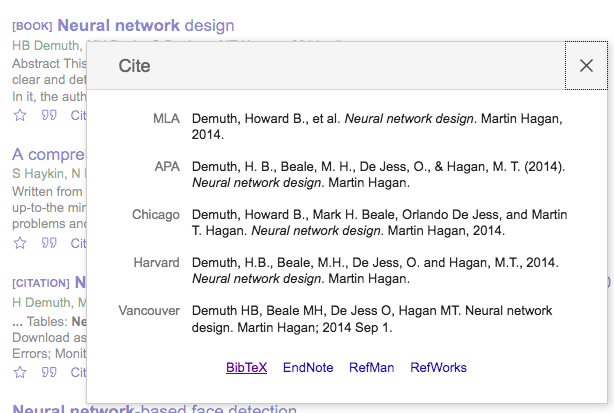
\includegraphics[width=0.45\textwidth]{bibtex.png}}
      \caption{Example of how to find the bibtex on Google Scholar. Click on the quotation marks, then select bibtex.}
      \label{fig:bibtex}
    \end{figure}
    \someundefinedcommand
\end{comment}


\section{Latex basics} \label{sec:latex}

By this point, you probably notice that latex is quite simple and intuitive. If you are curious about more, try consulting \url{http://www.stat.pitt.edu/stoffer/freetex/latex%20basics.pdf}.

For a short version of things to know, this template already cover the basics. Note how you can reference a section, figure, or table by using $\backslash ref\{\}$, refering to some $\backslash label\{\}$ you define elsewhere in the document.

Finally, this is how you define a table.

\section{Latex editor} \label{sec:editor}

There are many latex editor. One is MikTEX. There are also online tools called sharelatex \footnote{\url{https://www.sharelatex.com/}}. I recommend using this service since it require no installation. You can try for free but in order to use the more advance features (online collaboration and version control) you need to pay for its service. I have a paid subscription. If you want to use the online collaboration feature, contact me and I will host the project for your group.

\begin{table}
\centering
\begin{tabular}{|l|c|c|c|c|} % this defines how many columns and indentation of each column
 \hline % creates a horizontal line
First & 2nd & 3rd & 4th \\ %columns are separated by & and newline is \\
 \hline
 Phones & 28 & 48 & 38 \\
 Tones & n/a & n/a & n/a \\
 Graphemes & 27 & 57 & 28 \\
 Amount & 3 & 3 & 3 \\
 Wideband & yes & yes & yes \\
 Vocab & 3.7k & 7.3k & 5.4k \\
 Word count & 33k & 25k & 27k \\
 Speakers & 358 & 362 & 371 \\
 Web data amount & 38.0M & 6.4M & 16.2M \\
 \hline
\end{tabular}
\caption{Some table}
\label{tab:table}
\end{table}

% References should be produced using the bibtex program from suitable
% BiBTeX files (here: bibl_conf). The IEEEbib.bst bibliography
% style file from IEEE produces unsorted bibliography list.
% -------------------------------------------------------------------------
\bibliographystyle{IEEEbib}
\bibliography{conference}

\end{document}

